\chapter{\ifenglish Background Knowledge and Theory\else ทฤษฎีที่เกี่ยวข้อง\fi}

การการทําโครงงานเริ่มต้นด้วยการศึกษาค้นคว้าทฤษฎีที่เกี่ยวข้อง หรืองานวิจัย/โครงงานที่เคยมีผู้พัฒนาและนําเสนอไว้แล้ว ซึ่งเนื้อหาในบทนี้ก็จะเกี่ยวกับ
การอธิบายถึงทฤษฎีีที่นำไปประยุกต์ใช้กับโครงงานนี้ เพื่ออำนวยให้ผู้อ่านทำความเข้าใจกับตัวระบบของโครงงานได้ง่ายขึ้น

\section{You Only Look Once Object Detection Algorithm (YOLO)}
YOLO \cite{yolo} เป็นอัลกอริทึมสำหรับการระบุบริเวณที่สนใจภายในภาพ และจำแนกประเภทของวัตถุบนแต่ละบริเวณแบบเวลาจริงเหมือนกับตัวจำแนกภาพปกติ 
โดยที่ภาพหนึ่งสามารถประกอบด้วยบริเวณที่สนใจหลายบริเวณ แล้วแต่ละบริเวณจะนำไปจำแนกวัตถุที่แตกต่างกันได้ ซึ่งทำให้เกิดความซับซ้อนสูงในการ
จำแนกภาพระหว่างการตรวจจับวัตถุ ต่างจากอัลกอริทึมตรวจจับวัตถุทั่วไปที่จะใช้อัลกอริทึมแบบ Two-stage Object Detection YOLO 
นั้นจะใช้แบบ Single-shot Object Detection แทน ซึ่งใช้การสแกนภาพแต่ละภาพเพียงครั้งเดียวสำหรับการพยากรตำแหน่งของวัตถุที่ต้อง
การจะตรวจจับ และเนื่องจากการประมวลผลภาพเพียงครั้งเดียวนั้น ส่งผลให้อัลกอริทึมดังกล่าวใช้ระยะเวลาในการประมวลผลต่ำ 
เหมาะกับการนำไปใช้แบบเวลาจริง แต่ก็แลกมากับข้อเสียที่ความแม่นยำในการตรวจจับภาพนั้นอาจไม่มากเท่าอัลกอริทึมแบบ Two-stage Object Detection 
โดยใช้เทคนิคการเรียนรู้แบบ Convolutional Neural Network ดังรูปที่ 2.1
\begin{figure}[h]
  \begin{center}
  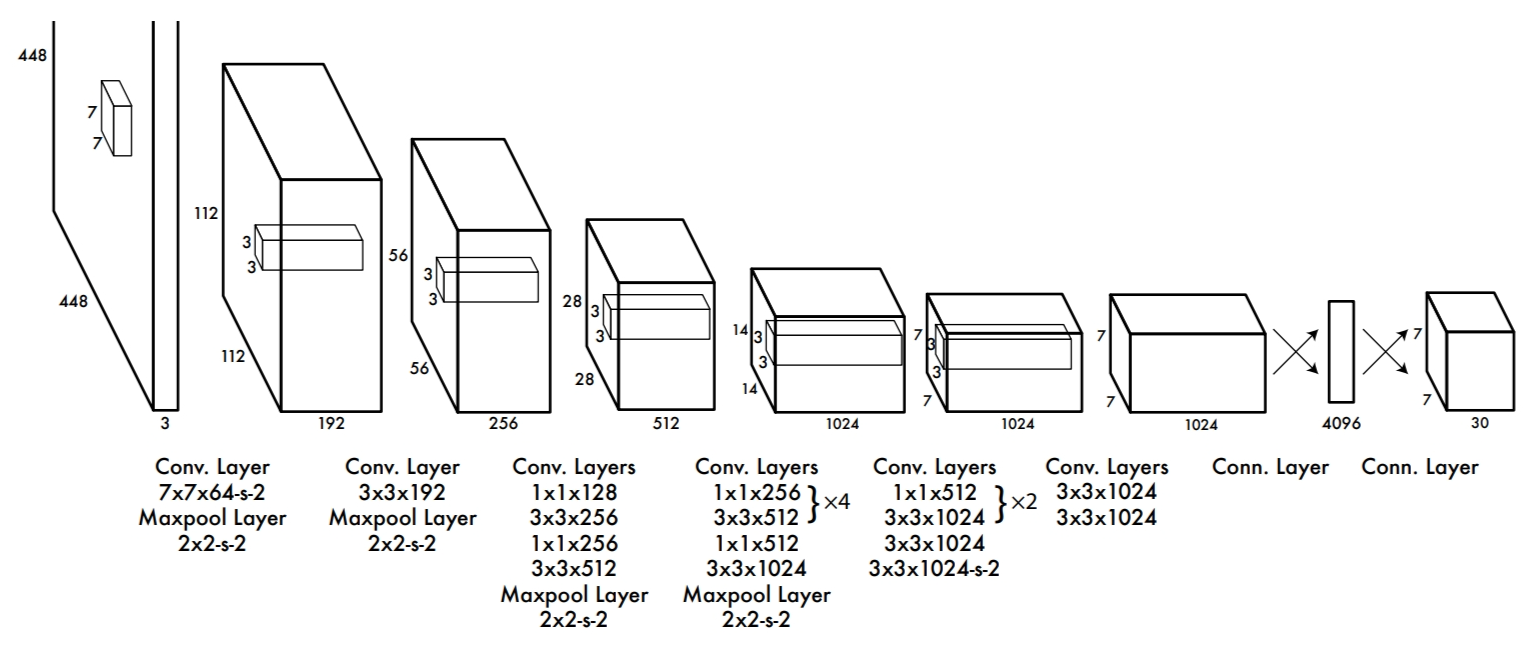
\includegraphics[scale=0.2]{resources/YOLO.png}
  \end{center}
  \caption[YOLO Architecture]{You Only Look Once Architecture}
  \label{fig:yolo architecture}
\end{figure}


\section{Object Relational Mapping (ORM)}
Object-Relational Mapping \cite{orm} เป็นการสร้างการสัมพันธ์ระหว่างฐานข้อมูลแบบ Relational กับโครงสร้างข้อมูลแบบ Object-Oriented 
ตามรูปที่ 2.2 ในการพัฒนาซอฟต์แวร์ เช่น เว็บแอปพลิเคชัน โดยที่ไม่ต้องเขียน SQL โดยตรงแต่สามารถใช้ภาษาโปรแกรมเพื่อจัดการกับข้อมูลแทน 
ซึ่งสามารถป้องกันการโจมตีแบบ SQL Injection ได้ ในกรณีที่กำหนดให้มีการเปลี่ยนแปลงในโครงสร้างข้อมูล 
คุณสมบัติหรือโครงสร้างข้อมูลในฐานข้อมูลจะถูกปรับเปลี่ยนตามในโครงสร้างของ Object ในโปรแกรม เป็นฐานข้อมูลแบบเสมือนในโปรแกรม 
โดยที่การจัดเก็บข้อมูลยังคงเป็นแบบ Relational เหมือนเดิม โดยไม่ต้องใช้ SQL Statements โดยตรง
\begin{figure}[h]
  \begin{center}
  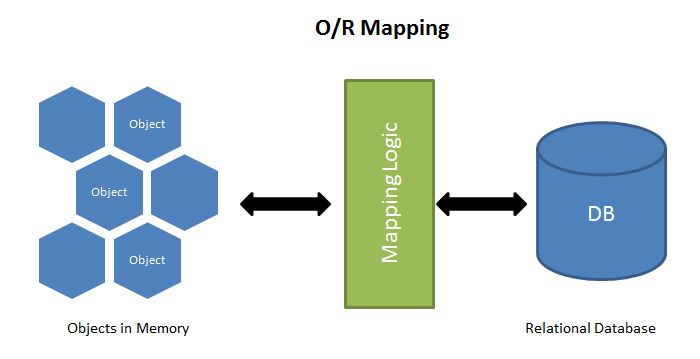
\includegraphics[scale=0.3]{resources/ORM.png}
  \end{center}
  \caption[Object Relational Mapping]{Object Relational Mapping}
  \label{fig:orm}
\end{figure}

\section{Model–View–Controller design pattern (MVC)}
Model-View-Controller \cite{mvc} เป็นรูปแบบโครงสร้างที่แยกแอปพลิเคชันออกเป็น 3 ส่วนหลักคือ: โมเดล (model), มุมมอง (view), 
และคอนโทรลเลอร์ (controller) แต่ละส่วนมีการสร้างขึ้นเพื่อจัดการด้านพัฒนาส่วนแอปพลิเคชันที่เฉพาะเจาะจง ตามรูปที่ 2.3 MVC 
เป็นหนึ่งในรูปแบบการพัฒนาเว็บตามมาตรฐานอุตสาหกรรมที่ถูกใช้บ่อยที่สุดเพื่อสร้างโครงงานที่สามารถเพิ่มและขยายขนาดในอนาคตได้ 
โดยที่ว่าเพื่อให้โปรแกรมนั้นดูเรียบง่ายต่อการแก้ไขจัดการ ซึ่งความหมายในแต่ละส่วนของ MVC นั้นได้แก่ 
\begin{enumerate}
  \item Model คือส่วนที่รับผิดชอบเกี่ยวกับข้อมูลและการประมวลผลทางด้านข้อมูลในแอปพลิเคชัน เช่น การเชื่อมต่อกับฐานข้อมูล การจัดการข้อมูล 
  และการประมวลผลทางข้อมูล เป็นต้น โดยที่ model มักจะเป็นตัวแทนของข้อมูลและสถานะของแอปพลิเคชัน
  \item View คือส่วนที่จะเป็นหน้าตาของโปรแกรมที่ผู้ใช้จะใช้งานจากส่วนนี้ ไม่ว่าจะเป็นการกรอกข้อมูล, ดูผลลัพธ์ หรือการมีปฏิสัมพันธ์กับผู้ใช้ 
  (User Interface) view จริง ๆ แล้วก็คือส่วนที่เรียกว่า GUI (Graphic User Interface) 
  \item Controller เป็นส่วนที่รับผิดชอบในการควบคุมและจัดการกับการกระทำที่เกิดขึ้นจากผู้ใช้งาน เช่น การรับข้อมูลจากผู้ใช้งาน, 
  การส่งข้อมูลไปยังโมเดลเพื่อประมวลผล, และการอัพเดตสถานะของ view ซึ่งโดยทั่วไปแล้ว controller จะเป็นตัวกลางที่เชื่อมต่อระหว่าง model 
  และ view โดยการควบคุมการทำงานของทั้งสอง 
\end{enumerate}
\begin{figure}[h]
  \begin{center}
  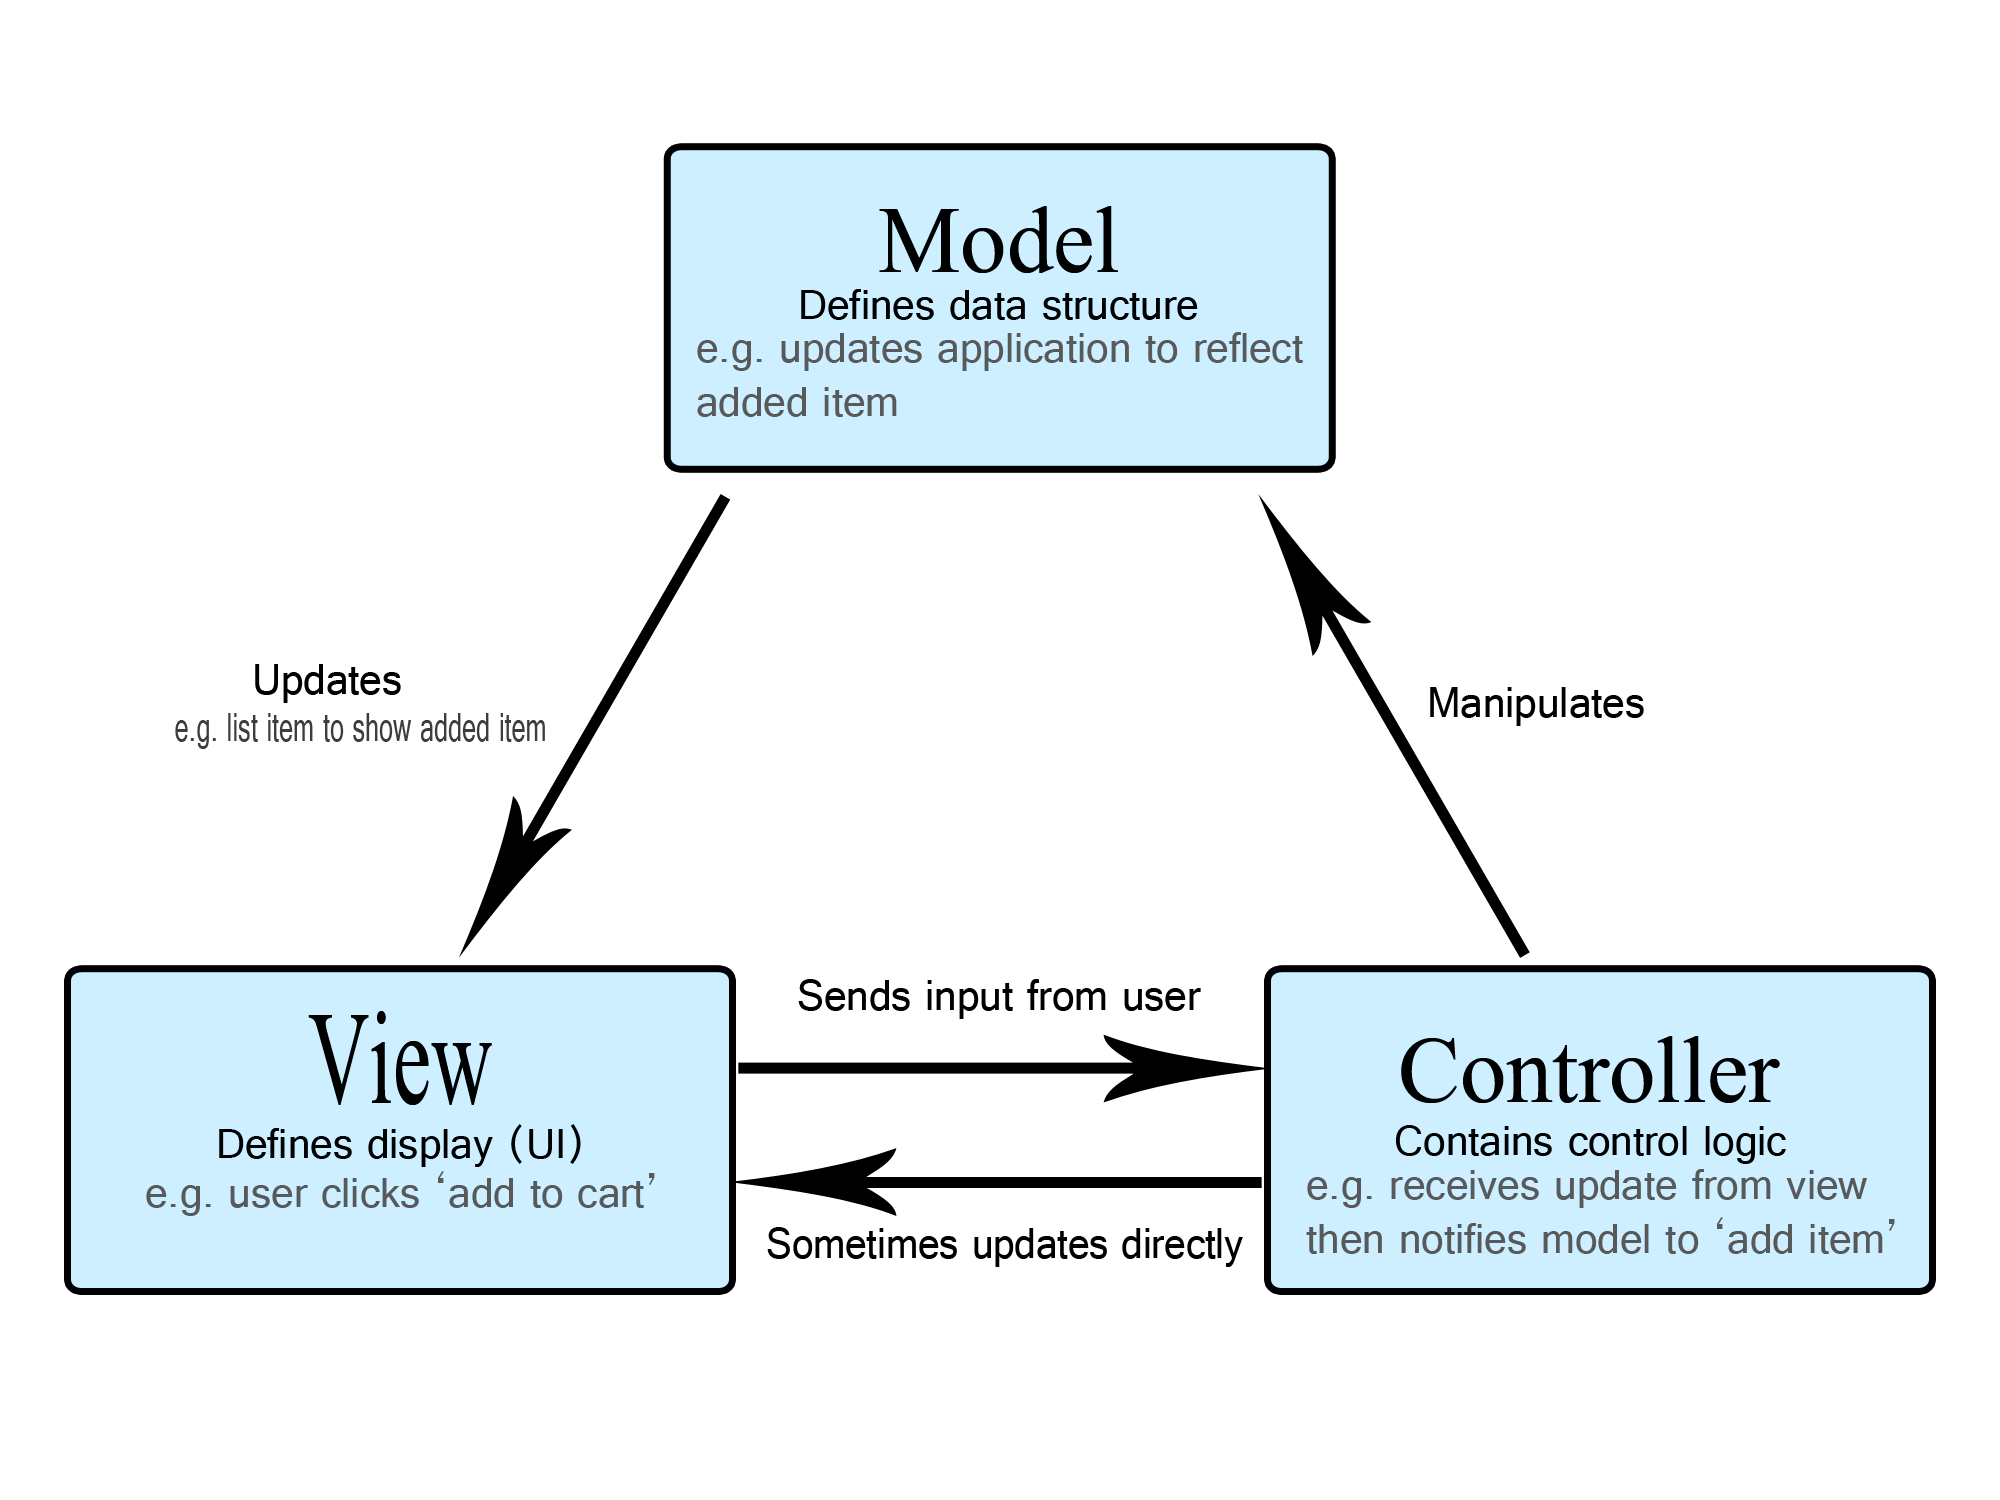
\includegraphics[scale=0.3]{resources/MVC.png}
  \end{center}
  \caption[Model-View-Controller]{Model-View-Controller Design Pattern}
  \label{fig:mvc}
\end{figure}

\section{Hypertext Transfer Protocol (HTTP)}
HTTP (Hypertext Transfer Protocol) เป็นโปรโตคอลสื่อสารที่ใช้ในการส่งข้อมูลระหว่างเครื่องคอมพิวเตอร์บนเครือข่ายอินเทอร์เน็ต โดย HTTP 
มีหน้าที่เป็นตัวกลางในการร้องขอและส่งข้อมูลระหว่างเว็บไซต์ (web servers) และเบราว์เซอร์ (web browsers) หรือแอปพลิเคชันอื่น ๆ 
ที่ใช้เครือข่ายอินเทอร์เน็ต 
\begin{itemize}
  \item API (Application Programming Interface) เป็นชุดของกฎและโครงสร้างข้อมูลที่กำหนดโดยโปรแกรมคอมพิวเตอร์เพื่อให้แอปพลิเคชันอื่น ๆ 
  สามารถสื่อสารและทำงานร่วมกันได้ ในเชิงพื้นฐาน API เป็นวิธีที่แอปพลิเคชันใช้เรียกใช้ฟังก์ชันหรือการบริการที่ให้มาจากแหล่งข้อมูลหรือบริการ
  ซึ่งอาจเป็นเซิร์ฟเวอร์เว็บ ฐานข้อมูล หรือแหล่งข้อมูลอื่น ๆ โดยทั่วไป API จะรองรับการร้องขอและการตอบกลับโดยใช้ฟอแมตที่เป็นรูปแบบมาตรฐาน เช่น 
  JSON (JavaScript Object Notation) หรือ XML (Extensible Markup Language) 
\end{itemize}

\section{Docker}
Docker \cite{docker} เป็นเทคโนโลยีคอนเทนเนอร์แพลตฟอร์มที่ช่วยในการสร้างและทำการงานร่วมกับคอนเทนเนอร์อย่างมีประสิทธิภาพ ด้วย Docker 
ผู้ใช้สามารถแยกแยะและแพคเกจแอปพลิเคชันพร้อมกับสิ่งที่เกี่ยวข้องทั้งหมด เช่น ไฟล์ ระบบปฏิบัติการ ไลบรารี และสิ่งอื่น ๆ 
ลงในคอนเทนเนอร์ได้อย่างเรียบง่าย โดยมีโครงสร้างการทำงานตามรูปที่ 2.4 ผู้ใช้สามารถสร้าง และรันคอนเทนเนอร์ได้โดยง่าย นอกจากนี้ Docker 
ยังช่วยลดปัญหาเกี่ยวกับสภาพแวดล้อมและการติดตั้งโปรแกรมที่ซับซ้อน ทำให้การพัฒนาและการทำงานของโปรแกรมมีประสิทธิภาพมากขึ้น 
\begin{figure}[h]
  \begin{center}
  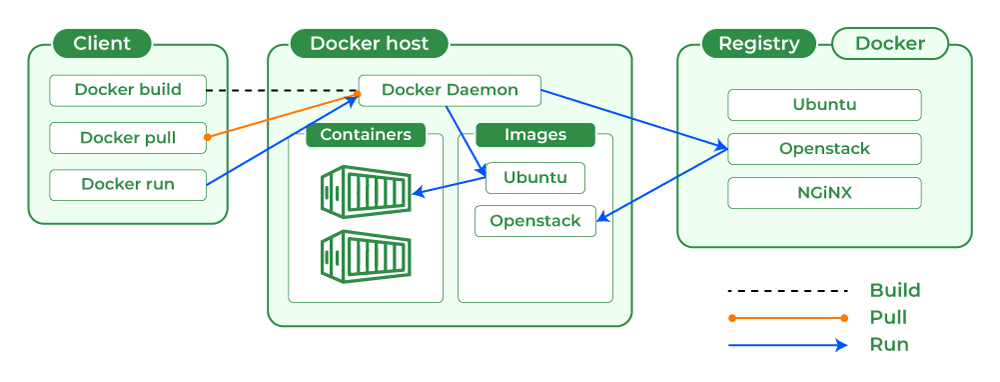
\includegraphics[scale=0.3]{resources/Docker.png}
  \end{center}
  \caption[Docker Architecture]{Docker Architecture}
  \label{fig:docker}
\end{figure}

\section{Interactive Website}
Interactive website \cite{interactive-web} คือ เว็บไซต์ที่สามารถให้ผู้ใช้งาน communicate หรือ interact เช่น การแสดงความคิดเห็น การตอบโต้กับตัวเว็บ 
การได้รับผลจากการกระทําในเว็บ ในลักษระที่เป็นมิตรต่อผู้ใช้ โดยปัจจุบัน มักใช้ animation sound picture audio etc. ประกอบ 
เพื่อให้มีความสนุกสนานและเพิ่มการเข้าถึงได้ง่ายของผู้ใช้ ทั้งนี้อาจทําเพื่อเก็บข้อมูลหลังจากการใช้งานเว็บไซต์ได้อีกด้วย ซึ่งดีกว่าเว็บที่มีแต่ตัวอักษร หรือ 
การแสดงผลเฉย ๆ ที่ได้รับข้อมูลทางฝ่ายเดียวอย่างแน่นอน

% \subsubsection{Subsubsection 1 heading goes here}
% Subsubsection 1 text

% \subsubsection{Subsubsection 2 heading goes here}
% Subsubsection 2 text

% \section{Third section}
% Section 3 text. The dielectric constant\index{dielectric constant}
% at the air-metal interface determines
% the resonance shift\index{resonance shift} as absorption or capture occurs
% is shown in Equation~\eqref{eq:dielectric}:

% \begin{equation}\label{eq:dielectric}
% k_1=\frac{\omega}{c({1/\varepsilon_m + 1/\varepsilon_i})^{1/2}}=k_2=\frac{\omega
% \sin(\theta)\varepsilon_\mathit{air}^{1/2}}{c}
% \end{equation}

% \noindent
% where $\omega$ is the frequency of the plasmon, $c$ is the speed of
% light, $\varepsilon_m$ is the dielectric constant of the metal,
% $\varepsilon_i$ is the dielectric constant of neighboring insulator,
% and $\varepsilon_\mathit{air}$ is the dielectric constant of air.

% \section{About using figures in your report}

% % define a command that produces some filler text, the lorem ipsum.
% \newcommand{\loremipsum}{
%   \textit{Lorem ipsum dolor sit amet, consectetur adipisicing elit, sed do
%   eiusmod tempor incididunt ut labore et dolore magna aliqua. Ut enim ad
%   minim veniam, quis nostrud exercitation ullamco laboris nisi ut
%   aliquip ex ea commodo consequat. Duis aute irure dolor in
%   reprehenderit in voluptate velit esse cillum dolore eu fugiat nulla
%   pariatur. Excepteur sint occaecat cupidatat non proident, sunt in
%   culpa qui officia deserunt mollit anim id est laborum.}\par}

% \begin{figure}[h]
%   \centering

%   \fbox{
%      \parbox{.6\textwidth}{\loremipsum}
%   }

%   % To include an image in the figure, say myimage.pdf, you could use
%   % the following code. Look up the documentation for the package
%   % graphicx for more information.
%   % \includegraphics[width=\textwidth]{myimage}

%   \caption[Sample figure]{This figure is a sample containing \gls{lorem ipsum},
%   showing you how you can include figures and glossary in your report.
%   You can specify a shorter caption that will appear in the List of Figures.}
%   \label{fig:sample-figure}
% \end{figure}

% Using \verb.\label. and \verb.\ref. commands allows us to refer to
% figures easily. If we can refer to Figures
% \ref{fig:walrus} and \ref{fig:sample-figure} by name in the {\LaTeX}
% source code, then we will not need to update the code that refers to it
% even if the placement or ordering of the figures changes.

% \loremipsum\loremipsum

% % This code demonstrates how to get a landscape table or figure. It
% % uses the package lscape to turn everything but the page number into
% % landscape orientation. Everything should be included within an
% % \afterpage{ .... } to avoid causing a page break too early.
% \afterpage{
%   \begin{landscape}
%   \begin{table}
%     \caption{Sample landscape table}
%     \label{tab:sample-table}

%     \centering

%     \begin{tabular}{c||c|c}
%         Year & A & B \\
%         \hline\hline
%         1989 & 12 & 23 \\
%         1990 & 4 & 9 \\
%         1991 & 3 & 6 \\
%     \end{tabular}
%   \end{table}
%   \end{landscape}
% }

% \loremipsum\loremipsum\loremipsum

% \section{Overfull hbox}

% When the \verb.semifinal. option is passed to the \verb.cpecmu. document class,
% any line that is longer than the line width, i.e., an overfull hbox, will be
% highlighted with a black solid rule:
% \begin{center}
% \begin{minipage}{2em}
% juxtaposition
% \end{minipage}
% \end{center}

% \section{\ifenglish%
% \ifcpe CPE \else ISNE \fi knowledge used, applied, or integrated in this project
% \else%
% ความรู้ตามหลักสูตรซึ่งถูกนำมาใช้หรือบูรณาการในโครงงาน
% \fi
% }

% อธิบายถึงความรู้ และแนวทางการนำความรู้ต่างๆ ที่ได้เรียนตามหลักสูตร ซึ่งถูกนำมาใช้ในโครงงาน

% \section{\ifenglish%
% Extracurricular knowledge used, applied, or integrated in this project
% \else%
% ความรู้นอกหลักสูตรซึ่งถูกนำมาใช้หรือบูรณาการในโครงงาน
% \fi
% }

% อธิบายถึงความรู้ต่างๆ ที่เรียนรู้ด้วยตนเอง และแนวทางการนำความรู้เหล่านั้นมาใช้ในโครงงาน
